\chapter{方案设计与实现}
\label{chap:design_implement}
%Overview
本章重点介绍基于Clearwater系统的网络功能服务链资源映射优化的设计和实现。在本设计中,需要结合底层运行平台运行时信息和具体服务请求来作为系统输入,生成之后的优化决策并映射到实际的物理系统中。当系统初始化时,本设计将物理平台的动态性能测试的结果作为运行时参数输入系统,后续算法将以该参数作为算法执行时的参照标准。当收到一个服务链的请求后,将上层抽象的业务需求转化为具体的服务链业务链表。系统的动态映射模块根据服务链的实际组成来映射相应的具体实例。在映射实例的过程中,本设计的原型平台Clearwater默认使用的是随机映射的策略,而这种策略在实际的运行环境中缺乏对服务链中所涉及的虚拟机和所分配的底层资源的感知。本设计在第\ref{chap:model}章所提出的模型基础上,使用基于底层性能信息的优化算法生成新的映射策略替代默认的随机映射策略,从而提升资源的利用效率和网络服务的性能。

\section{总体设计概述}
\subsection{总体设计目标}
一个有效的资源映射策略应当在服务功能完整的前提下进行资源的有效配置。在服务器中,数据从一个网络功能节点传输到另一个节点的过程中不可避免的会产生传输的延迟,数据传输的带宽也会因为底层不同数据路径的原因有所差别。服务器平台的处理器数量和内存空间也是有限的,不平衡的负载分布会导致剧烈的资源竞争甚至导致意想不到的性能下降。因此,本文所设计的系统需要考虑到以上各个因素,生成相对优化的资源映射策略。在本文中,设计主要关注以下的三个目标:
\begin{enumerate}
	\item 有效的资源映射策略应当首先保证网络功能服务链的完整性。在对物理资源进行资源分配时应保证服务链中功能节点的完整性,能够提供有效的网络服务。
	\item 有效的资源映射策略应该能够提升在使用相同数量物理资源下的服务性能。
	\item 有效的资源映射策略应当考虑实际的负载分布,避免因为局部负载过高而产生的性能下降。
\end{enumerate}

\subsection{总体设计思路}
鉴于已有验证性实验的观测结论和以上对此类问题的目标分析,本文所设计的系统需要获取实际服务链的具体组成结构,并考虑具体实例之间物理资源的数据传输性能来满足实际应用的最小带宽和最大延迟要求,同时在保证服务完整性的前提下提升物理资源的利用效率。

为了实现以上的设计目的,本设计提供了一种基于底层多核运行平台的虚拟化网络功能的映射方法。首先,当平台接受到一个服务请求时,应当根据服务请求的解析来确认所需要的网络功能组和具体提供服务的网络功能服务链。本设计会评估当前服务资源是否满足提供服务的最小需求,即组成服务链的不同功能组中是否有足够的运行实例。当资源充足时,系统开始根据参与服务链具体功能实例来组织服务。在挑选具体服务实例时,系统根据预先处理生成的物理资源数据传输性能矩阵作为调度算法的输入,根据矩阵中资源间互相访问的性能大小关系和当前机器的负载信息,依照网络功能服务链的连接顺序,使用局部最优的方法搜索构造出相对较优的服务链与实例的映射关系,根据所挑选出的实例来组织网络功能服务链。

\subsection{总体设计架构}

基于上文所提的设计思路,本文提出了一套底层运行平台感知的优化系统。该系统架构如图\ref{fig:system}所示,本系统设计了两个模块来实现前文中的设计目标:\textbf{信息采样模块}和\textbf{动态映射模块}。

\textbf{信息采样模块}使用标准的采样工具动态获取服务器物理资源间的数据传输性能信息。这些不同物理核之间的数据传输带宽和延迟信息可以反映在NUMA架构平台下物理资源的实时传输性能,为动态映射模块利用优化算法生成映射结果提供具体的数据参数,并且该模块还实时监控当前系统的负载情况为生成映射策略提供负载信息。

\textbf{动态映射模块}收到组链请求后,根据服务请求的类别来确定所参与服务的功能实例组,并通过本文所提出的基于贪心的优化算法,以信息采样模块的数据作为输入参数,挑选服务收益较高的功能组实例来组成服务链响应服务。下文中将具体介绍信息采样模块和动态映射模块的模块设计与实现。通过这两个模块的数据传递和协同合作,实现优化资源映射策略的生成和注入,从而达到设计目标。

\begin{figure}[!htp]
	\centering
	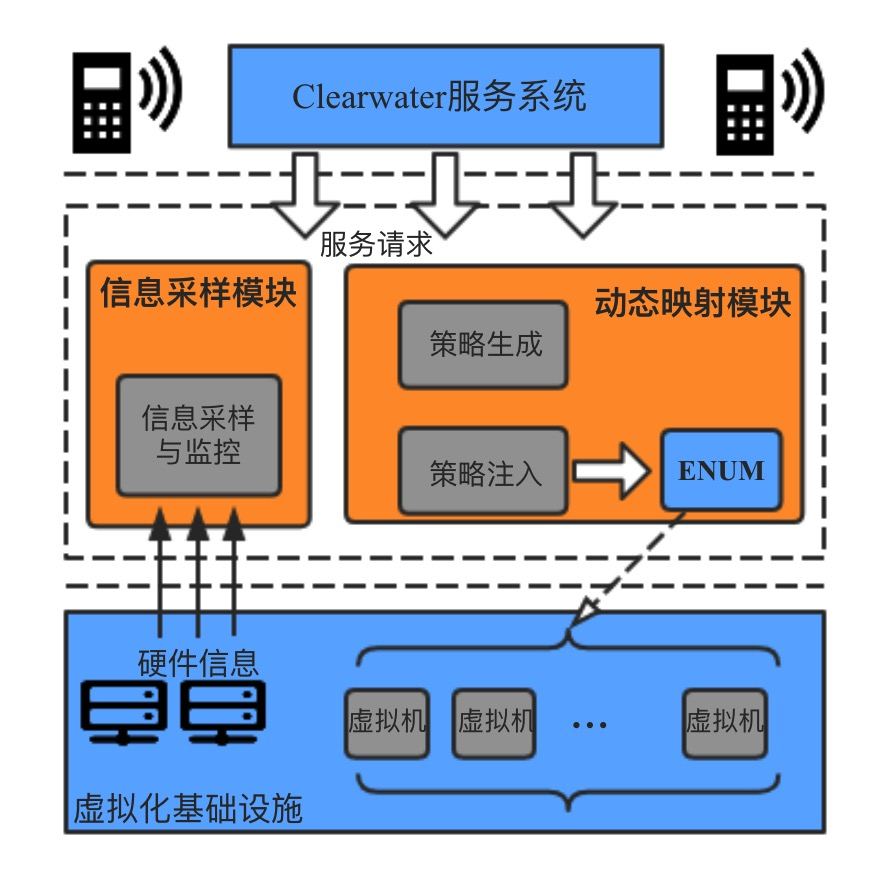
\includegraphics[width=0.8\textwidth]{system.jpg}
	\bicaption[fig:system]{映射优化系统架构示意图}{映射优化系统架构示意图}{Fig}{Overview of the Optimization System}
\end{figure}

\newpage

\section{子模块设计与实现}
\subsection{Clearwater服务链分析} 
为了保证设计系统的完整性目标,本节首先对Clearwater的服务链进行分析并确定各种服务所需的服务功能组,在保证
服务完整性的前提下优化Clearwater服务的资源映射。Clearwater平台的核心功能服务包括:\textbf{用户注册流程},\textbf{初始化拨号流程},\textbf{通话流程}和\textbf{通话终止流程}。根据总结的服务流程和对应的服务链,将每个服务链以链表的形式记录下来存储到预定义的配置文件中。当收到某一类服务请求时,根据服务请求类型在预定义的文件中选择对应的服务链功能实例组,完成服务链服务分析。完整的服务链分析如图\ref{fig:clearwater_sfc}所示,各流程的完整描述如下:

\textbf{用户注册流程}{ }当客户端发起注册请求时,Sprout节点将从Dime节点中获取认证信息,如果没有相关认证记录则请求拒绝, Sprout节点同时缓存该请求记录,一旦后续出现相同请求则直接处理不再查询。如果查询到相关认证记录认证通过,则向客户端返回认证成功。如果有第三方认证,则跳转到第三方登记流程。该流程主要涉及到的网络功能节点为Bono,Sprout和Dime。

\textbf{初始化拨号流程}{ }该流程主要参与的网络功能有Sprout、Homestead当客户端向Sprout节点发起通话请求,Sprout节点通过HTTP请求从Homestead节点缓存中获取拨号者和被拨号信息,同时生成本次服务的iFC\footnote{http://www.3gpp.org/ftp/Specs/archive/29\_series/29.228/29228-b70.zip appendices B and F}。随后Sprout向ENUM组件中查询所拨打用户是否在线,如果在线则 Sprout完成查询终止iFC,并根据查询结果向被拨打者发起SIP INVITE请求,同时向 AS(Vellum) 中记录SIP Ringing状态。当被拨叫客户端接听后,返回SIP 200 OK,则通过Sprout节点更新AS (Vellum)记录。整个过程中所涉及到的功能节点为:Bono,Sprout和Dime。

\textbf{通话流程}{ }客户端通过Sprout不断在通话过程中不断更新状态信息到 AS(Vellum) 中,更新数据同样通过Sprout反馈到被叫客户端中。整个过程中所涉及到的功能节点为:Bono,Sprout,Vellum。

\textbf{通话终止流程}{ }当通话结束后,客户端发起挂断请求,Sprout将状态存储到 AS(Vellum) 中,并向被拨号者发起SIP BYE请求,请求响应后同样更新 AS(Vellum)记录,返回SIP 200 OK,通话终止。整个过程中所涉及到的功能节点为:Bono,Sprout,和Vellum。

\begin{figure}[!htp]
	\centering
	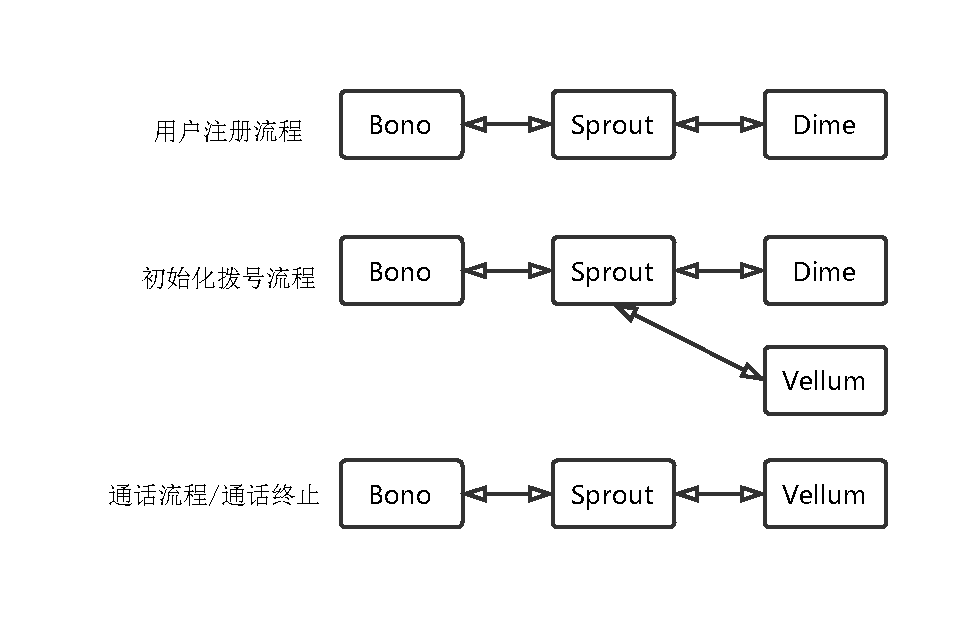
\includegraphics[width=0.8\textwidth]{service.pdf}
	\bicaption[fig:clearwater_sfc]{Clearwater核心业务服务链}{Clearwater核心业务服务链}{Fig}{Core SFCs of Clearwater System}
\end{figure}

根据本小节中对平台核心服务的分析,可以获得核心服务请求所对应的具体功能组以及服务链结构,动态映射模块将根据具体服务链结构进行映射策略的生成,从而保证所生成的服务的功能完整性。

\subsection{信息采样模块}
\label{imp:sample}

信息采样模块负责从底层硬件获取运行平台架构信息和运行时各处理器节点的数据传输性能信息。在高性能的NUMA服务器上,先前的研究主要使用跳距离来量化不同物理核间的数据传输性能。跳距离是高级配置与电源接口(Advanced Configuration and Power Interface, ACPI)定义的代表NUMA节点间的距离信息。我们可以使用numactl\footnote{https://linux.die.net/man/8/numactl}工具获取当前的机器的NUMA节点之间的距离信息。但是仅仅获取这样的信息不足以满足第\ref{chap:model}章中提出的模型所需的带宽和延迟信息。因此在信息采样模块中,本文提出通过预处理采样的方式将获取的带宽和延迟信息存储在矩阵 $D$ 中,元素 $D_{i,j}$ 表示当使用第 $i$ 号CPU访问在位于 $j$号CPU时,所需要的带宽和延迟信息。该矩阵的大小和具体物理平台的处理器数量相关,即服务器有N个CPU时,该矩阵大小为$N\times N$。

%\begin{figure}[!htp]
%	\label{fig:numactl}
%	\centering
%	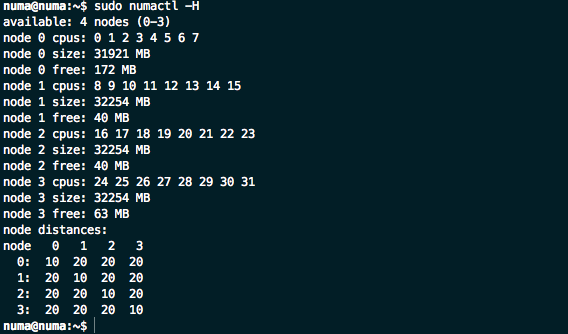
\includegraphics[width=0.8\textwidth]{numactl.png}
%	\bicaption[fig:numactl]{使用numactl工具获取NUMA距离信息}{使用numactl工具获取NUMA距离信息}{Fig}{numactl overview}
%\end{figure}

$$
D =
\begin{pmatrix}
10      & 8      & \cdots & 4      \\
9      & 10      & \cdots & 5      \\
\vdots & \vdots & \ddots & \vdots \\
4      & 3      & \cdots & 10     \\
\end{pmatrix}
$$
同时,该模块还负责对运行平台进行实时的监控和信息反馈,获取服务器当前的负载状态来作为动态映射模块的实时输入参数。

为了满足如上设计中对底层平台信息的实时采样,本文使用经典的内存访问测试工具Stream 和 Intel Memory Latency Checker作为采样工具,预先运行并获取所有运行时参数,作归一化处理后分别存入如上的信息矩阵中。本文所使用的平台有32个物理核,即可以得到两个$32\times32$的矩阵。所生成的信息参考矩阵被以文件的形式存储在系统硬盘上,供动态映射模块读取。

为了获取当前平台的实时负载信息,信息采样模块使用了一个动态的节点负载的监测工具。通过加载系统msr模块\footnote{http://man7.org/linux/man-pages/man4/msr.4.html}来调用PCM \footnote{https://software.intel.com/en-us/articles/intel-performance-counter-monitor} 工具动态地监测每个物理核当前的负载信息。监测模块每秒更新一次并将结果输出至文件中。本文中重点关注如表格 \ref{tab:dynamic} 中所列出的信息,其中主要选取L3 cache的命中率将作为当前处理器节点的负载参考指标,将这个信息输入作为算法\ref{alg:greedy}中参数$\phi$的实际值。

\begin{figure}[!htp]
	\centering
	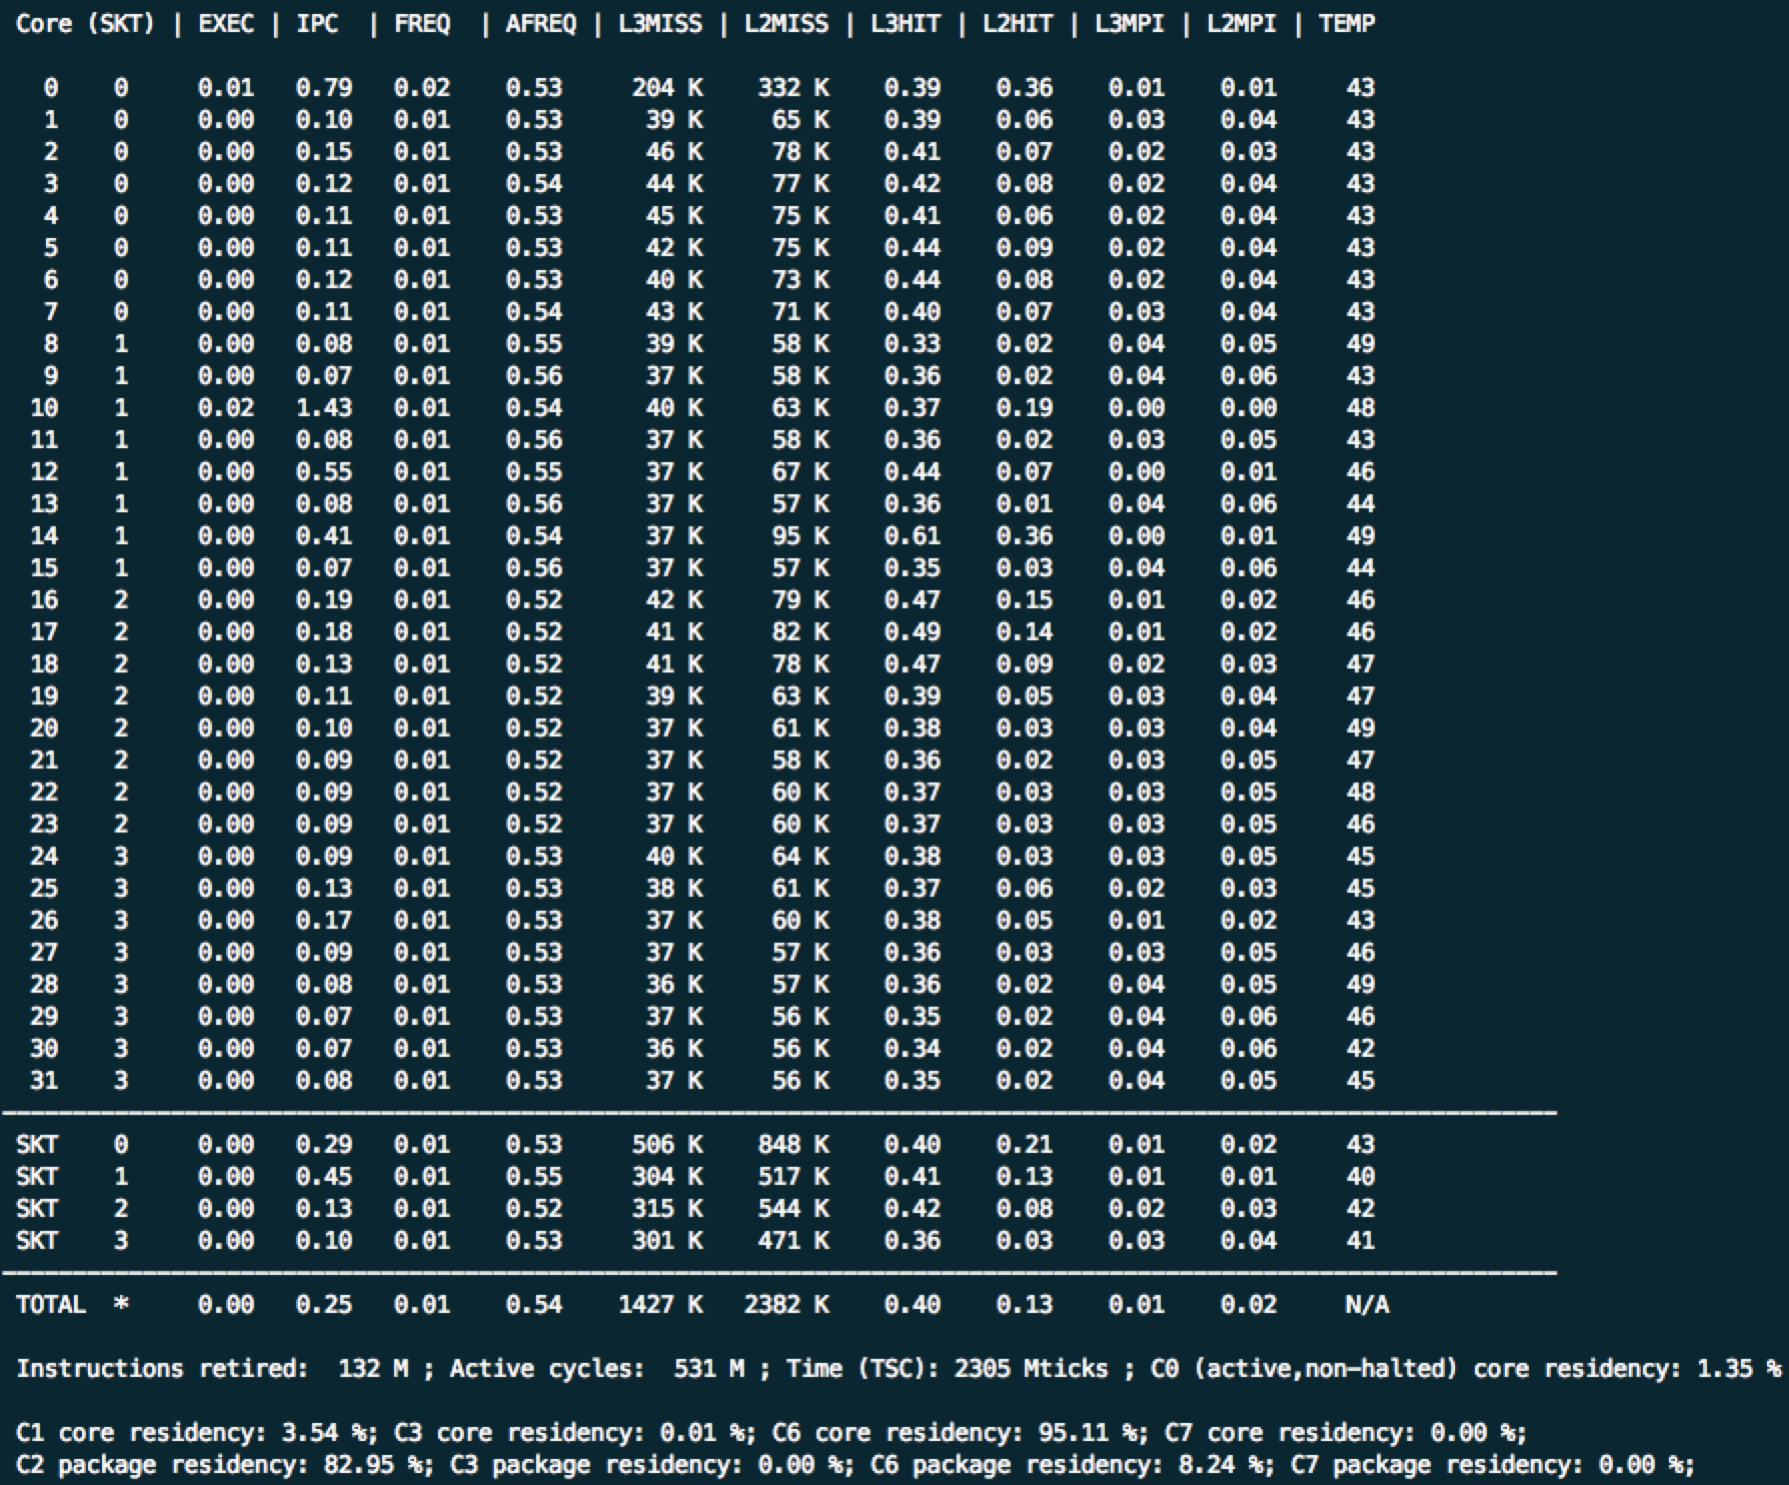
\includegraphics[width=0.8\textwidth]{pcm.png}
	\bicaption[fig:PCM]{使用PCM工具获取运行时负载信息}{使用PCM工具获取运行时负载信息}{Fig}{Using PCM Tool Monitoring System Real-time Workload}
\end{figure}

\begin{table}[!htb]
	\centering
	\bicaption[tab:dynamic]{服务器实时监测参数}{服务器实时监测参数}{Table}{Table of State Parameters of Running Server}
	\begin{tabular}{ | l | p{7cm} |}\hline
		\textbf{参数} &							 \textbf{参数涵义}  				\\ 	\hline
		IPC   & 当前CPU周期指令数\\ \hline
		L3MISS & L3 cache未命中次数\\ \hline
		L2MISS & L2 cache未命中次数\\ \hline
		L3HIT & L3 cache 命中率 (0.00-1.00)\\ \hline
		L2HIT & L2 cache 命中率 (0.00-1.00)\\ \hline
		L3MPI & 每个指令周期内的L3cache miss数\\ \hline
		L2MPI & 每个指令周期内的L2cache miss数\\ \hline
		READ  & 内存读取数 (GBytes)\\ \hline
		WRITE & 内存写入数 (GBytes)\\ \hline
	\end{tabular}
\end{table}


\subsection{动态映射模块}
动态映射模块主要负责服务链资源映射策略生成和策略的部署。在该模块中,本设计按照服务链分析中所总结的各种服务类型,通过算法\ref{alg:greedy}映射成为具体的实例链表,并根据实例链表完成服务链的组建,生成对应的映射策略。根据生成的映射策略,覆盖平台原有的实例选择方法,完成映射过程。整个过程如图\ref{fig:flow}所示。从整体架构上分析,实现本文中所设计动态映射模块包括以下关键步骤:

步骤1、对底层平台进行预处理,获得与平台底层运行时相关的信息矩阵。与普通从硬件中读取参数不同,通过动态采样的方法获取平台运行时实时性能参数能更加准确地反映底层平台的架构差异以及所引起的性能差异。首先,动态采样可以实现与操作系 统无关性能信息获取,不管多核平台运行的操作系统版本如何,都可以通过采样程序获 取该操作系统下的实时运行结果。其次,相比于直接从主板芯片中读取多核架构中不同处理器节点的预定义信息,动态采样的方法通过动态地运行测试程序,可以获得更加接 近实际情况的量化数据。基于这样的数据信息,可以更加准确地刻画底层物理资源之间 的数据传输性能。最终信息被存进格式化的信息矩阵中,作为步骤2的输入。

步骤2、当一条服务请求到来时,分析该请求所对应的服务链。

步骤3、根据请求所对应服务链的数据流向确定所需要的虚拟网络功能服务点,

步骤4、使用基于贪心的方法并依照信息矩 阵中的参数生成映射决策序列来确定待映射的具体运行实例,进入步骤5。

步骤5、根据步骤4生成映射的实例序列,依次检查实例在对应的物理资源节点当前的负载情况,如果某一实例所在节点的负载过高,增加负载会加剧资源竞争导致当前运行实例的性能下降,则返回步骤4将本次的映射序列标记为失效,重新生成新的实例映射序列。检查通过后进入步骤6。

步骤6、根据生成的映射序列,替代默认的随机选取策略,实现优化后的服务链到实际物理资源的映射。


\begin{figure}[!htp]
	\centering
	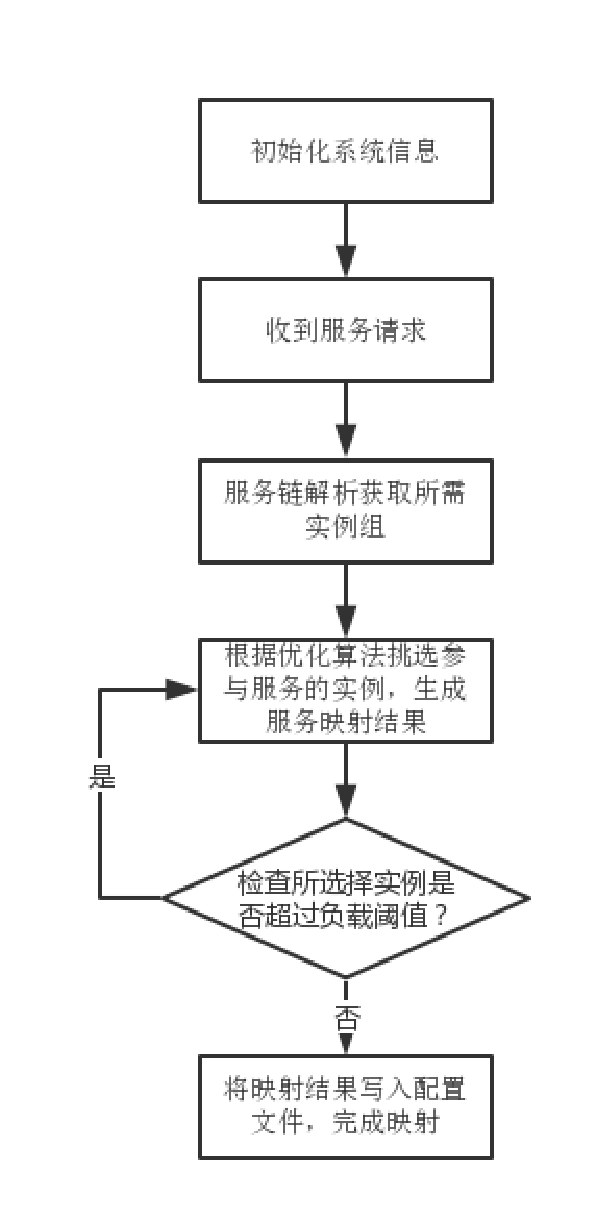
\includegraphics[width=0.4\textwidth]{coordinator.pdf}
	\bicaption[fig:flow]{动态映射模块工作流程}{动态映射模块工作流程}{Fig}{Flow of Coordinator Module Working Procedure }
\end{figure}\textbf{}

\subsubsection{基于贪心的映射算法}
在上文建立的基于IMS服务链资源映射模型基础上,本小节主要介绍了在这样的应用场景下的一种基于贪心的资源映射策略算法。本设计的映射策略如算法\ref{alg:greedy}所示。本文提出两种基于贪心思想的映射策略。第一种是基于服务链上任意两个相邻节点具有最大通信带宽的最大带宽策略 (GMB, Greedy Maximum Bandwidth),第二种是任意两个相邻节点具有最小通信延迟的最小延迟策略 (GML, Greedy Minimum Latency)。但带宽和延迟这两个影响因素同时可以提高整体映射策略的收益时,这两种策略可以同时被用于同一个服务链的映射生成。如果被映射的服务需要较高的通信带宽并根据其带宽来衡量其服务质量,例如数据传输服务,那么这种服务就适合使用GMB算法来生成映射结果;如果服务链的服务质量是由整体的通信延迟所决定的,那么GML便更适合这类的应用场景。这两种算法通过收益函数中的系数来具体调节。

算法 \ref{alg:greedy} 的具体步骤如下:服务链请求被解析成对应服务链链表输出后,算法 \ref{alg:greedy} 将该链表 $L$ 作为算法输入,顺序遍历该链表,针对链表中每个元素$i$,利用公式 \ref{equ:profit} 计算其收益函数,从待选实例中筛选出收益最大的实例并判断该实例所在计算节点的 L3cache 命中率,若未命中的比例超过 90\% 则放弃该实例选择次优收益的实例并继续比较其cache的命中率,直到有合适的实例被选中为止,将被选中实例加入结果链表$L^{\prime}$中。当筛选流程完后,检查$L^{\prime}$,若链表为空,则映射失败,否则根据链表中所选取的实例来组织相应的服务链。通过以上的算法 \ref{alg:greedy},理论上我们可以选择出相对收益最高的服务链与实例的映射链表。算法的输出结果将作为输入传入动态映射模块,该模块将根据该结果进行服务链组链操作。
%TODO 修改为语言描述
%\begin{algorithm} 
%	\caption{基于贪心的映射策略}  
%	\label{alg:greedy}  
%	\begin{algorithmic} [1]
%		\State Start
%		\State Input List $L$ of SFC $S$
%		\State Backup Substrate Network State
%		\For{ Function $i \in L$}
%		\State Initialize: Capable Instances Set $L^{\prime} = \emptyset$
%		\For{ Node $j \in D$} \RComment Got max P from all nodes in the function domain D
%		\State	$P = \max(\alpha*B_{j} + \beta*L_{j})$ 
%		\If {$\phi < 90\% $ }
%		\State $L^{\prime} = L^{\prime}\uplus j$
%		\Else { Delete selected node from $D$ and Pick new node with max P}
%		\EndIf			
%		\EndFor					
%		\If {$L^{\prime} \equiv \emptyset$}
%		\State Mapping Failed
%		\State Reset Substrate Network Status
%		\Return
%		\EndIf
%		\State Sort $L^{\prime}$ according to $L$	
%		\State Select the top node $j^{\star}$ from $L_{\prime}$
%		\State Map the function $i$ onto  $j^{\star}$
%		\State Update $D_{j}$.
%		\EndFor
%		\State Mapping Completed
%		\State End
%	\end{algorithmic}  
%\end{algorithm} 

\begin{algorithm} 
	\caption{基于贪心的映射策略}  
	\label{alg:greedy}  
	\begin{algorithmic} [1]
	\State Start
	\State Input List $L$ of SFC $S$
	\State Backup Substrate Network State
	\State Initialize: Capable Instances Set $L^{\prime} = \emptyset$
	\State //初始化结果集
	\For{ Function $i \in L$}	
	\State Randomly Select the Instance of the Head Element of $L$ 
	\State//随机选取服务链初始实例.
	\State Calculate $P = \alpha*Bandwidth(L^{\prime}) + \beta*(Latency(L^{\prime}))$ 
	\State//根据第三章模型中的公式考虑每个实例的服务带宽和延迟,计算$D$中所有可用实例的服务收益。$\alpha$,$\beta$ 分别为带宽和延迟的调节参数。
	\State Select the Instance with Max Value of $P$ 
	\State//选取收益最大的实例作为备选实例。
	\State Get L3 Cache Miss Rate $\phi$ of Selected Instance
	\If {$\phi < 90\% $ }
	\State $L^{\prime} = L^{\prime}\uplus j$
	\Else { Delete Selected Instance from $D$ and Pick New One}
	\State//如果负载参数$\phi$超过阈值,则从$D$中删除此实例,重新按照上述步骤挑选新备选实例
	\EndIf	
	\State $L^{\prime} = L^{\prime}\uplus j$							
	\If {$L^{\prime} \equiv \emptyset$}
	\State Mapping Failed
	\State Reset Substrate Network Status
	\Return
	\EndIf
%	\State Sort $L^{\prime}$ According to $L$.	
	\EndFor
	\State Map the Function and Update $D$.
	\State End
	\end{algorithmic}  
\end{algorithm} 
\newpage

\subsubsection{映射策略生成}
\begin{lstlisting}[title=Coordinator.java, frame=shadowbox]
```
final public  Map<Integer,VNF> getOptimumMapping(SFC sfc){
	ArrayList<VNF_TYPE> descriptor = sfc.getSFCDescriptor();//获取所需要的映射的服务链
	Map<Integer, VNF> result = new HashMap<>();

	Integer nextCpuId = -1;//初始化数据
	Integer preCpuId = -1;
	Integer curCpuId = -1;
	Double  curLoad = 0.0
	
	for (VNF_TYPE type:descriptor) {
		int optimalChose = Integer.MAX_VALUE;
		VNF nextVNF = null;
		for (VNF vnf : runningVNFs) {
			if (vnf.getType() == type && vnf.isIdle) {
				//随机选取服务链中第一个网络功能
				if(curCpuId < 0) {
					curCpuId = vnf.getVcpuNumber();
					preCpuId = curCpuId;
					vnf.setIdle(false);
					result.put(curCpuId,vnf);
					break;
				}
				curCpuId = vnf.getVcpuNumber();
				if (latancyMatrix[preCpuId/8][curCpuId/8] < optimalChose){
					optimalChose = latancyMatrix[preCpuId/8][curCpuId/8];
					nextCpuId = curCpuId;
					nextVNF = vnf;
				}
			}
		}
		curLoad = getL3CacheMiss(nextCpuId); //获取所选取节点的L3CacheMiss率作为负载参考。
	if(nextCpuId != -1 && curLoad < 0.9 ) result.put(nextCpuId, nextVNF);
	}
	return result;
```
}
\end{lstlisting}

在初始化阶段将所有的实例具体信息录入系统,包括其具体的网络功能、所分配的物理资源信息以及详细的配置参数。当有服务请求到来时,根据具体的业务请求来解析并翻译成该服务的响应服务链。此时动态映射模块根据算法\ref{alg:greedy}生成具体的映射策略,核心实现方法见上文中的Coordinator.java文件所示。

\subsubsection{映射策略注入}
具体的映射策略生成后,接下来需要实现具体的映射策略注入操作。我们从实例列表中将所选出的实例的ip提出,通过修改Clearwater的Sprout节点中的 \textit{/etc/clearwater/enum.json} 文件和绑定规则,可以实现服务链的动态修改。平台提供了两种修改绑定的方式,分别为利用 BIND 服务或者 dnsmasq 服务。本设计使用 BIND 服务来修改DNS绑定,具体的配置文件如图\ref{fig:enum}所示,并按照\textit{<enum domain name> <order> <preference> <flags> <service> <reg-exp>}的语法规则来添加相应服务。当服务映射规则更新到配置文件中之后,Clearwater系统会按照更新后的解析规则来选取实例完成组链,提供相应的服务功能。通过动态映射模块的从策略生成到配置文件修改这一些列操作,完成IMS服务链的动态组建。

\begin{figure}[!htp]
	\centering
	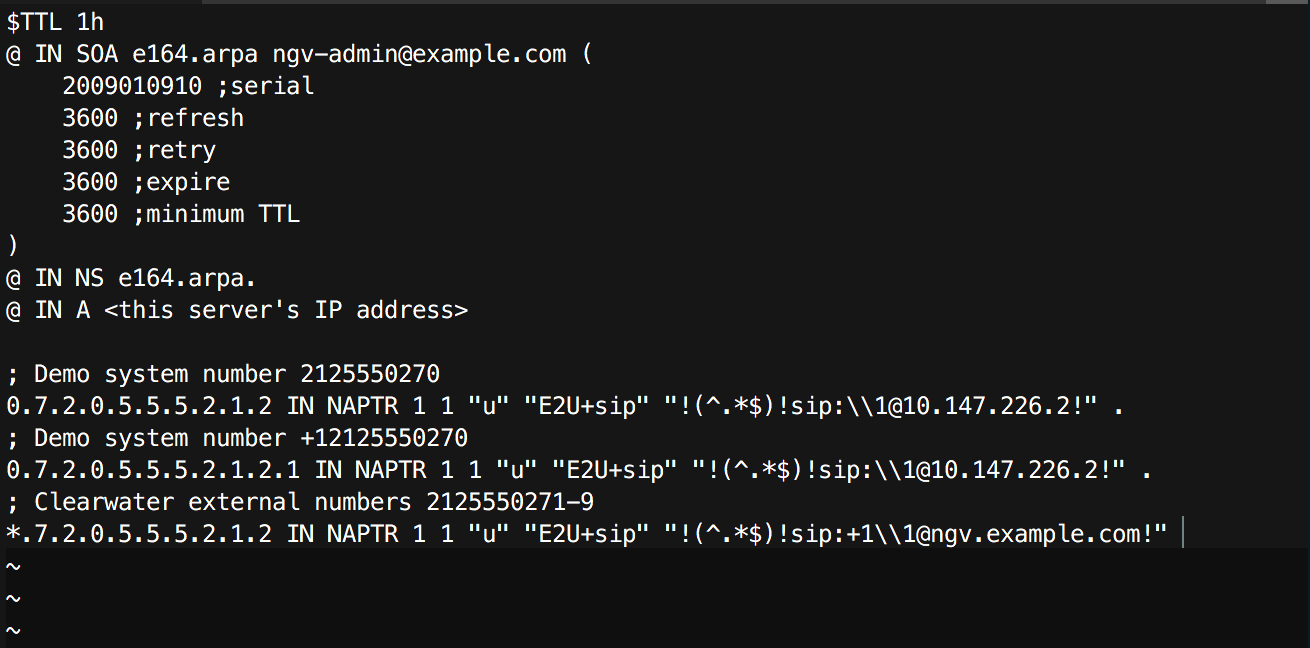
\includegraphics[width=0.8\textwidth]{enum.png}
	\bicaption[fig:enum]{Enum配置文件信息}{Enum配置文件信息}{Fig}{Enum configuration overview}
\end{figure}

经过动态映射模块重新组建的服务链在虚拟资源的数据传输性能上充分考虑了底层运行平台的NUMA特性,通过结合信息采样模块中所获取的运行时带宽和延迟信息,生成优化后的虚拟资源映射组合来提供相应的服务。
\newpage
\section{本章小结}
本章主要介绍了基于Clearwater平台的优化资源分配实现方法的设计与实现,主要包括本设计的设计目标、设计思路以及详细的模块设计分析与实现。在所建立模型的基础上,本文提出了设计的所关注的三个目标,并以这些目标作为约束详细阐述了本文的总体设计思路和模块的设计细节。最后,详细介绍了平台的总体算法以及底层信息采样模块和动态映射模块的一些实现细节信息。